\section{Discussion}
To compare the discussed methods Figure \ref{f:Comparison} classifies them qualitatively with respect to the attributes \textit{accuracy of uncertainty propagation} and \textit{computational efficiency}. The ground-truth trajectory sampling scales cubicly but is highly accurate. The Gaussian approximation approach with Taylor expansion accounts for the propagation of uncertainty while only scaling quadratically. The computational complexity is further decreased with the independence assumption but at the cost of accuracy. The same is true for the basis function approximation that scales linearly but is again incaccurate. The posterior split method on the other hand combines an accurate representation of the uncertainty plus it only scales linearly with the prediction horizon.
\begin{figure}[ht]
        \centering
        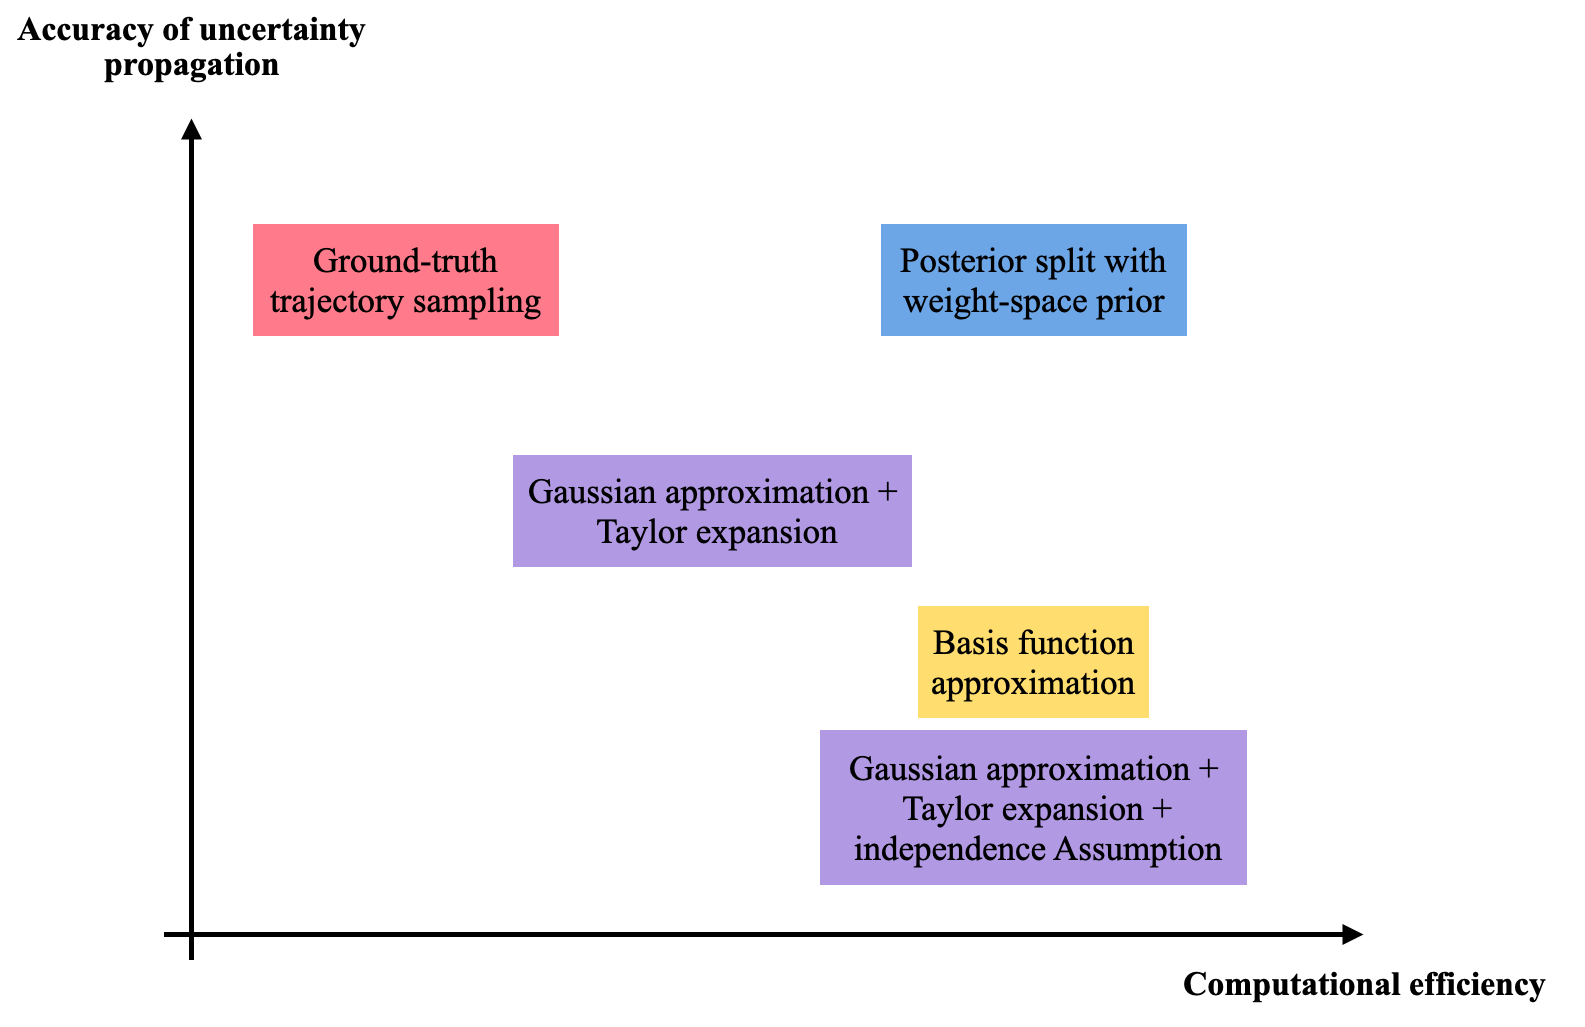
\includegraphics[width=1.1\linewidth]{SoM_report_template/figures/Bildschirmfoto 2020-12-18 um 12.50.51.png}
        \caption[Qualitative comparison of methods]{\label{f:Comparison} Qualitative comparison of methods }
\end{figure}

\section{Conclusion}
In conclusion there are many methods proposed in the literature to deal with the drawbacks of GPs, specifically lack of scalability and inaccurate approximations of uncertainty propagation. While they all improve on the naive trajectory sampling (\ref{naiveapprox}) they differ in computational cost and accuracy. The method that stands out is the combination of function-space and weight-space interpretation (\ref{eq:GPPosteriorSplit}), as it both preserves the uncertainty propagation and scales only linearly with the prediction horizon. 